\documentclass[tikz,border=10pt]{standalone}
\usepackage{tikz-3dplot}
\usepackage{amsmath, amssymb}
\usetikzlibrary{arrows.meta, positioning, calc, decorations.pathreplacing, 3d}
\usetikzlibrary{matrix, fit, backgrounds, shapes}
\usetikzlibrary{angles,quotes}

\usepackage[T1]{fontenc}
\usepackage[utf8]{inputenc}
\usepackage{newpxtext,newpxmath}
\usepackage{sectsty}

\begin{document}
%========================================================
% TikZ #4 (Step 4): apply (alpha,beta)->(alpha,-beta) to get T(p)
%========================================================
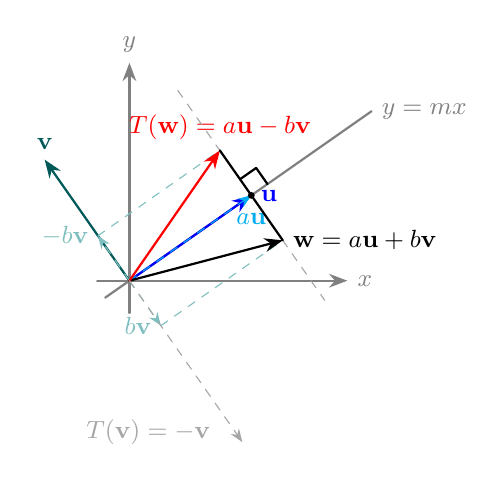
\begin{tikzpicture}[scale=2.05, >=Stealth, line cap=round, line join=round]
	\def\m{0.7}
	\def\px{0.95}
	\def\py{0.25}
	
	% u=(1,m), v=(-m,1)
	\pgfmathsetmacro{\ux}{1}
	\pgfmathsetmacro{\uy}{\m}
	\pgfmathsetmacro{\vxB}{-\m}
	\pgfmathsetmacro{\vyB}{1}
	
	\pgfmathsetmacro{\den}{1+(\m)^2}
	\pgfmathsetmacro{\alpha}{(\px + \m*\py)/\den}
	\pgfmathsetmacro{\beta}{(-\m*\px + \py)/\den}
	
	% Key points
	\coordinate (P)  at (\px,\py);
	\coordinate (AU) at ({\alpha*\ux},{\alpha*\uy});          % alpha u
	\coordinate (BV) at ({\beta*\vxB},{\beta*\vyB});          % beta v
	\coordinate (mBV) at ({-\beta*\vxB},{-\beta*\vyB});       % -beta v
	
	% p = AU + BV,   T(p)= AU + (-BV)
	\coordinate (Psum)  at ({\alpha*\ux+\beta*\vxB},{\alpha*\uy+\beta*\vyB});      % should equal P
	\coordinate (TP)    at ({\alpha*\ux-\beta*\vxB},{\alpha*\uy-\beta*\vyB});
	
	% midpoint M between p and T(p)
	\pgfmathsetmacro{\mx}{(\px + (\alpha*\ux-\beta*\vxB))/2}
	\pgfmathsetmacro{\my}{(\py + (\alpha*\uy-\beta*\vyB))/2}
	\coordinate (M) at (\mx,\my);
	
	%======================
	% STYLES
	%======================
	\tikzset{
		axis/.style={thick, gray},
		axline/.style={thick, gray},
		uvec/.style={thick, blue},
		vvec/.style={thick, teal!70!black},
		pvec/.style={thick, black},
		tvec/.style={thick, red},
		comp/.style={dashed, gray!70, ->},
		help/.style={dashed, gray!70},
		box/.style={rounded corners, draw=gray!60, fill=white, inner sep=3pt},
		mat/.style={font=\small}
	}
	
	\newcommand{\panelaxes}{
		\draw[axis,->] (-0.2,0) -- (1.35,0) node[right] {\small $x$};
		\draw[axis,->] (0,-0.2) -- (0,1.35) node[above] {\small $y$};
	}
	
	\newcommand{\rightangleat}[3]{% X,Y,size
		\coordinate (RAU) at ({#1 + #3},{#2 + #3*\m});     % along axis
		\coordinate (RAN) at ({#1 - #3*\m},{#2 + #3});     % along normal
		\coordinate (RAC) at ({#1 + #3 - #3*\m},{#2 + #3*\m + #3});
		\draw[thick] (RAU) -- (RAC) -- (RAN);
	}
	
%	\node[box, anchor=west] at (-0.2,1.38) {\small Step 4: apply $(\alpha,\beta)\mapsto(\alpha,-\beta)$};
	
	\panelaxes
	
	% reflection axis
	\draw[axline] (-0.15,{-0.15*\m}) -- (1.5,{1.5*\m})
	node[pos=1, right] {\small $y=mx$};
	
	% basis vectors (short)
	\draw[uvec,->] (0,0) -- ({0.75*\ux},{0.75*\uy}) node[pos=1, right] {\small $\textbf{u}$};
	\draw[vvec,->] (0,0) -- ({0.75*\vxB},{0.75*\vyB}) node[pos=1, above]  {\small $\textbf{v}$};
	
	% components: alpha u, beta v, -beta v
	\draw[comp, cyan] (0,0) -- (AU) node[pos=1, below=3pt] {\small $a\textbf{u}$};
	\draw[comp, teal!50] (0,0) -- (BV) node[pos=1, left] {\small $b\textbf{v}$};
	\draw[comp, teal!50] (0,0) -- (mBV) node[pos=1, left] {\small $-b\textbf{v}$};
	
	% parallelogram for p = AU + BV
	\draw[help, cyan] (AU) -- (P);
	\draw[help, teal!50] (BV) -- (P);
	
	% parallelogram for T(p) = AU + (-BV)
	\draw[help, cyan] (AU) -- (TP);
	\draw[help, teal!50] (mBV) -- (TP);
	
	% p and T(p)
	\draw[pvec,->] (0,0) -- (P)  node[pos=1, right] {\small $\textbf{w}=a\textbf{u}+b\textbf{v}$};
	\draw[tvec,->] (0,0) -- (TP) node[pos=1, above]  {\small $T(\textbf{w})=a\textbf{u}-b\textbf{v}$};
	
	% segment p--T(p), midpoint, normal, right angle
	% normal through M (perpendicular to axis)
	\draw[help] ({\mx-0.65*\m},{\my+0.65}) -- ({\mx+0.65*\m},{\my-0.65});
	\draw[thick] (P) -- (TP);
	\fill (M) circle (0.6pt);
	
	% right angle marker at M
	\rightangleat{\mx}{\my}{0.10}	
	
	\draw[help,->] (0,0) -- ({-\vxB},{-\vyB}) node[pos=0.80, below left] {\small $T(\textbf{v})=-\textbf{v}$};
	
%	\node[anchor=west, mat] at (-0.18,1.05) {Flip the perpendicular component: $\beta v\mapsto -\beta v$.};
\end{tikzpicture}
\end{document}